\chapter{Isoviscous elastic-plated  gravity current model  for shallow
  magmatic intrusion}

\label{chap2} 
\minitoc

\citet{Michaut:2011kg} proposed a model for the spreading of a shallow
depth intermediate-size intrusion, in which magma is continuously
injected  at the  center and  is accommodated  by the  bending of  the
overlying strata.  In particular, the model differs from previous ones
by considering both the dynamics of the emplacement itself, in a sense
that the radius is self-consistently determined, and the driving force
associated with the magma weight. Both were neglected in previous models.
In  the  original paper  from  \citet{Michaut:2011kg},  the model  was
derived in  both cartesian and  axisymmetric geometry and  the results
were presented  in $2D$.  A similar  model in $2D$ with  an additional
fracture criterion  at the tip  of the  intrusion has been  derived by
\citet{Bunger:2011cb}  and  \citet{Anonymous:QWXp_4JV} discussed  more
precisely  the  dynamics at  the  contact  line  and  the case  of  an
elastic-plated gravity  current spreading over an  inclined plane.  In
this chapter,  we present a summary  of the model and  the results for
the spreading of  an isoviscous elastic-plated gravity  current over a
rigid horizontal  surface in  an axisymmetrical geometry.   Results in
this geometry  have been  thoroughly studied  by \citet{Lister:2013ia}
and this model will constitute the reference for more elaborate models
in the manuscript.

\section{Theoretical model}
\label{C2-sec:model}

The model considers an isoviscous elastic-plated gravity current, i.e.
an  isoviscous  fluid  of  viscosity  $\eta_h$  and  density  $\rho_m$
spreading beneath a thin elastic sheet  of thickness $d_c$ and above a
semi infinite rigid layer \citep{Michaut:2011kg,Bunger:2011cb} (Figure
\ref{C2-Sketch}).  The fluid is injected  continuously at the base and
center of the current at a rate $Q_0$ through a cylindrical conduit of
diameter $a$.

\begin{figure}[h!]
  \begin{center}
    \graphicspath{ {/Users/thorey/Documents/These/Manuscript/Figure/Chapter2/} }
    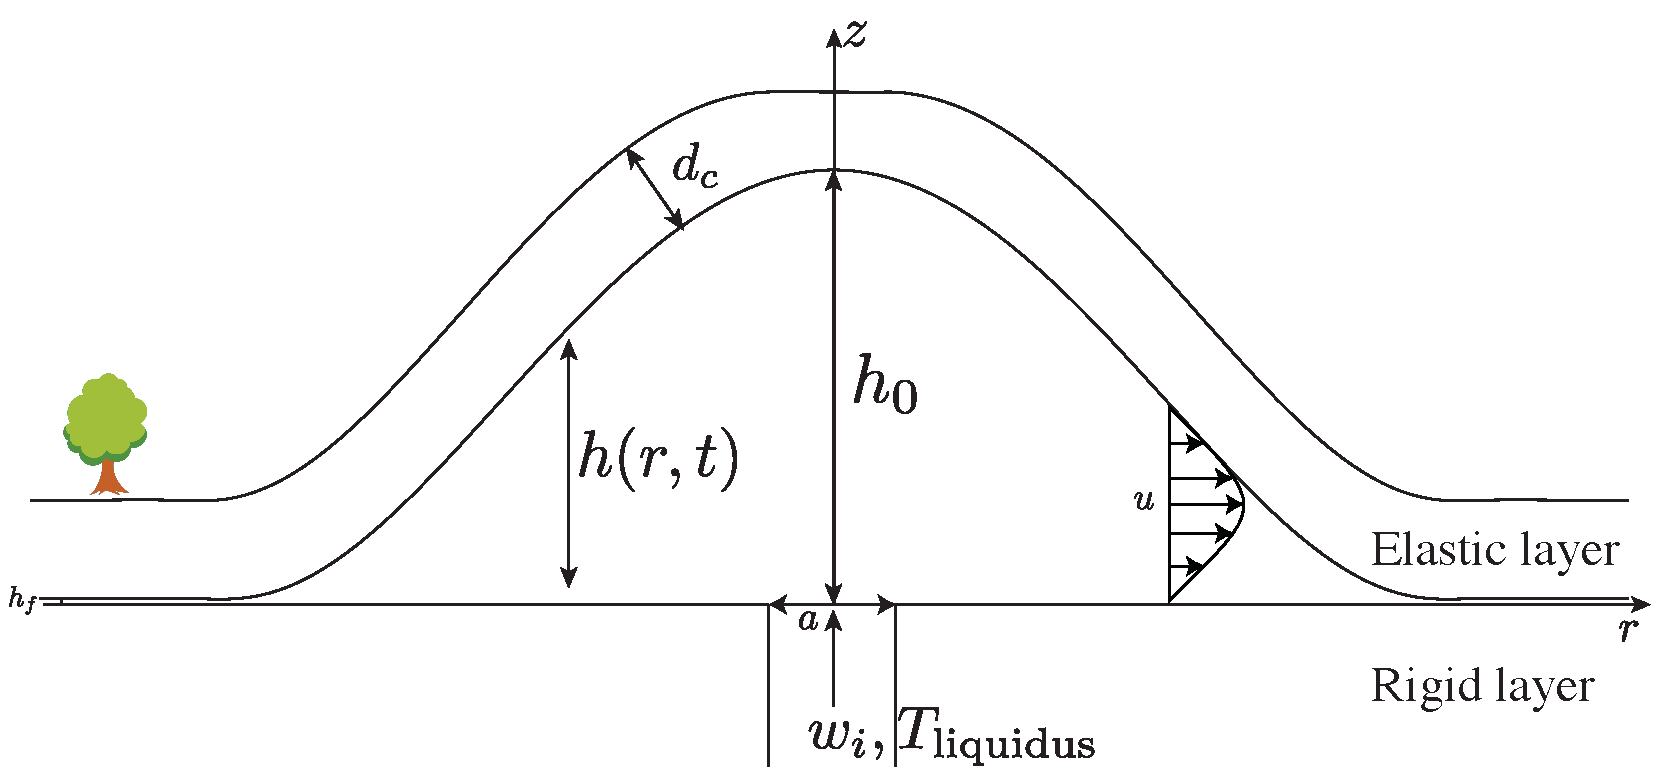
\includegraphics[scale=0.40]{C2_Sketch.pdf}
    \caption{Model geometry and parameters.}
    \label{C2-Sketch}
  \end{center}
\end{figure}

\subsection{Governing equation}
\label{C2-sec:Governing equation}

\textbf{Driving pressure}\\

The  intrusion develops  over a  length scale  $\Lambda$ that  is much
larger than its  thickness $H$ ($\epsilon = H/ \Lambda<<  1$).  In the
laminar  regime  and  in  axisymmetrical  coordinates  ($r$,$z$),  the
Navier-Stokes equations within the lubrication assumption are
\begin{eqnarray}
  -\frac{\partial P}{\partial r}  +  \frac{\partial}{\partial z}\left(\eta_h \frac{\partial u}{\partial z}\right) &=&0\label{C2_V1} \\
  -\frac{\partial P}{\partial z}  - \rho_{m}g&  =&0\label{C2-Npressure}
\end{eqnarray}
where  $u(r,z,t)$  is  the  radial   velocity,  $g$  is  the  standard
acceleration due to gravity and  $P(r,z,t)$ is the pressure within the
fluid.   Integration  of  (\ref{C2-Npressure}) thus  gives  the  total
pressure  $P(r,z,t)$ within  the flow.   When the  vertical deflection
$h(r,t)$ of the upper elastic layer is small compared to its thickness
$d_c$, i.e $h<<d_c$, we can neglect  stretching of the upper layer and
only  consider  bending  stresses.    Therefore,  the  total  pressure
$P(r,z,t)$  at  a level  $z$  in  the intrusion  is  the  sum of  four
contributions: the  weight of the  magma and  of the upper  layer, the
bending pressure $P_b$ and the atmospheric pressure $P_0$
\begin{equation}
  P = \rho_m g (h-z)+\rho_rgd_c+P_b+P_0
  \label{C2-pression}
\end{equation}
where $h(r,t)$ is the intrusion  thickness and $\rho_r$ the density of
the surrounding rocks. The bending pressure  is given by the force per
unit area  that is necessary  for a  vertical displacement $h$  of the
thin elastic plate \citep{Turcotte:1982ca}
\begin{equation}
  P_d = D\nabla_r^4h
\end{equation}
where $D$  is the flexural  rigidity of  the thin elastic  layer, that
depends on the Young's modulus $E$, Poisson's ratio $\nu^*$ and on the
elastic           layer          thickness           $d_c$          as
$D = Ed_c^3/\left(12(1-\nu^*^2)\right)$.

\vspace{.5cm} \textbf{Velocity field} \vspace{.5cm}

At the contact with the elastic sheet $z=h(r,t)$, the no-slip boundary
condition  hold and  then, the  tangential  velocity is  zero and  the
normal velocity  is the change  in height ($\partial h/  \partial t$).
With $\vec{n}$ the normal to the surface and $\vec{t}$ the tangent, we
have
\begin{eqnarray}
  \vec{n} \cdot (u,w) &=& \frac{\partial h }{\partial t}\\
  \vec{t} \cdot (u,w) &=& 0 \label{C2-tangeant}.
\end{eqnarray}
The  tangent  vector is  $\vec{t}  =  (1,  \partial h/  \partial  r)$.
However, within the lubrication  assumption, the vertical component of
the  tangent  vector scales  as  $\epsilon$  and thus,  is  negligible
compared to  the radial  component. Therefore, the  boundary condition
(\ref{C2-tangeant}) reduces  to $u(r,z=h,t) =0$.   At the base  of the
flow, the same boundary condition holds and $u(r,z=0,t) =0$.

Equation (\ref{C2_V1}) is integrated twice  as a function of $z$ using
these boundary conditions and the horizontal velocity is
\begin{equation}
  u(r,z,t) =\frac{1}{2\eta_h} \frac{\partial P}{\partial r} \left(z^2-hz\right).
  \label{C2-vel}
\end{equation}

\vspace{.5cm} \textbf{Injection rate} \vspace{.5cm}

The effective overpressure $\Delta P^*$ driving the flow in the feeder
conduit decreases as the intrusion thickens and is given by
\begin{equation}
  \Delta P^* = \Delta P -\rho_m g h_0 \label{C2-Q0}
\end{equation}
where $h_0(t)$ is the maximum  intrusion thickness at the center $r=0$
and $\Delta P$ is the initial  driving pressure or the overpressure at
the base of the dyke ($z = -Z_c$).

In (\ref{C2-Q0}), the bending pressure  at the center, which scales as
D$h_0(t)/R(t)^4$  where  $R(t)$  is   the  current  radius,  has  been
neglected.  Although  it tends  to infinity at  the initiation  of the
flow, it rapidly  vanishes as the current spreads  and the hydrostatic
pressure $\rho_m g h_0$ becomes  the main contribution to the pressure
at the  center.  In addition, the  model assumes a large  aspect ratio
for the flow and does not consider the initiation of the flow itself.

Finally,  assuming a  Poiseuille flow  within the  cylindrical feeding
conduit, the vertical injection velocity $w_i(r,t)$ and injection rate
$Q(t)$ are given by
\begin{equation}
  w_i=
  \begin{cases}
    \frac{ \Delta P^*}{4 \eta_h Z_{c}} (\frac{a^{2}}{4}-r^{2})& r \le \frac{a}{2}\\
    0 & r > \frac{a}{2}
  \end{cases}
  \label{C2-eq12}
\end{equation}
\begin{equation}
  Q = Q_0(1-\frac{\rho_m g h_0}{\Delta P})
  \label{C2-eq11}
\end{equation}
where
$Q_0=\left(\pi \Delta P^* a^{4}\right)/\left(128 \eta_h Z_c\right)$.

\vspace{.5cm} \textbf{Mass conservation} \vspace{.5cm}

The fluid  is assumed  incompressible and a  global statement  of mass
conservation gives
\begin{eqnarray}
  \frac{\partial         h}{\partial        t} +\frac{1}{r}
  \frac{\partial}{\partial
  r} \left( r\int_0^hudz\right) = w_i.
  \label{C2-Mass}
\end{eqnarray}
Injecting  (\ref{C2-vel})  into  (\ref{C2-Mass}),  we  find  that  the
equation for the evolution of the thickness in time and space reads
\begin{equation}
  \frac{\partial h}{\partial t} =\frac{\rho_mg}{12 \eta_h r}
  \frac{\partial}{\partial r}  \left( rh^3  \frac{\partial h}{\partial
      r}\right)+\frac{D}{12\eta_h r} \left( rh^3 \frac{\partial}{\partial r}\nabla_r^4h\right)+
  w_i .\label{C2-Heq}
\end{equation}
It is  composed of three different  terms on the right  hand side. The
first term represents gravitational  spreading, i.e.  spreading of the
current under its own weight. The second term represents the squeezing
of the  flow by the upper  elastic layer.  Both term  are negative and
induces spreading.   The last term  represents fluid injection  and is
positive.

\subsection{Dimensionless equations}
\label{C2-sec:dimens-equat}

Equation (\ref{C2-Heq}) is nondimensionalized using a horizontal scale
$\Lambda$, a vertical scale $H$ and a time scale $\tau$ given by
\begin{eqnarray}
  \Lambda &=& \left(\frac{D}{\rho_m g}\right)^{1/4}\label{C2-L1}\\
  H&=&\left       (\frac{12\eta_h      Q_{0}}{\rho_{m}g       \pi}\right      )
       ^{\frac{1}{4}} \label{C2-H1}\\
  \tau&=&\frac{\pi \Lambda^{2} H}{Q_{0}}\label{C2-T1}
\end{eqnarray}
in which scales are chosen such  that $Q_0 = \pi\Lambda^2 H/\tau$. The
length scale $\Lamba$ represents the  flexural wavelength of the upper
elastic layer,  i.e. the  length scale at  which bending  stresses and
gravity  equally contribute  to flow.   The  height scale  $H$ is  the
thickness of  a typical gravity current  and the time scale  $\tau$ is
the  characteristic time  to  fill  up a  cylindrical  flow of  radius
$\Lambda$ and thickness  $H$ at constant rate $Q_0$.   In addition, we
can       define        a       horizontal        velocity       scale
$U=\Lambda/\tau=\left(\rho_m           g           H^3\right)/\left(12
  \eta_h\Lambda\right)$.

The dimensionless equation is
\begin{eqnarray}
  \frac{\partial h}{\partial t}& =&\frac{1}{ r}
                                    \frac{\partial}{\partial r}  \left( rh^3  \frac{\partial h}{\partial
                                    r}\right)+\frac{1}{ r} \left( rh^3
                                    \frac{\partial}{\partial
                                    r}\nabla_r^4h\right)\nonumber\\
                               &+&
                                   \frac{32}{\gamma^{2}}\left(\frac{1}{4}-\frac{r^{2}}{\gamma^{2}}\right)\left(1-\frac{h_0}{\sigma}\right)
                                   \label{C2-mainEq}
\end{eqnarray}
where the last term is replaced by zero for $r>\gamma/2$. $\gamma$ and
$\sigma$ are two dimensionless numbers controlling the dynamics of the
flow
\begin{eqnarray}
  \gamma &=& \frac{a}{\Lambda}\\
  \sigma &=& \frac{\Delta P}{\rho_m g H}.
\end{eqnarray}
$\gamma$  is the  dimensionless radius  of  the conduit,  it does  not
significantly influence the flow and is set to $0.02$ in the following
\citep{Michaut:2009jx,Michaut:2011kg}.   $\sigma$  is  the  normalized
pressure  head,  i.e.,  the  ratio between  the  initial  overpressure
driving the flow and the weight of the magma at the center.
	 
\subsection{Need for regularization}
\label{C2-sec:need-regularization}

One  of   the  main   mathematical  difficulty  in   solving  equation
(\ref{C2-mainEq}) arises at the  contact line.  Indeed, the assumption
that the  thickness of  the fluid  tends to zero  at the  contact line
leads       to       divergent      viscous       stresses,       i.e.
$\eta_h  \partial  u/\partial  z\rightarrow  \infty$  and  hence,  the
theoretical         immobility          of         the         blister
\citep{Flitton:1999iv,Lister:2013ia,Anonymous:QWXp_4JV}. This problem,
known  a  the  contact-line  paradox,  is  a  well  know  problem  for
surface-tension driven flow  such as the spreading of  a water droplet
\citep{Bertozzi:1998wz,Snoeijer:2013cm}.

The formal proof  have been derived by  \citet{Flitton:1999iv} and can
be derived  as follow. Suppose  that (\ref{C2-mainEq}) has  a solution
and the solution has the  form $h \sim A(t)(R(t)-r)^{\alpha}$ near the
contact line.  As $r \rightarrow R(r)$, the bending term dominates the
gravitational term and (\ref{C2-mainEq}) reduces to
\begin{eqnarray}
  \frac{\partial       h}{\partial       t}&      =&\frac{1}{       r}
                                                     \frac{\partial}{\partial r}\left( rh^3 \frac{\partial}{\partial r}\nabla_r^4h\right).
                                                     \label{C2-mainEq2}
\end{eqnarray}
Injecting the  solution into  (\ref{C2-mainEq2}) and keeping  only the
leading powers of $R-r$ gives
\begin{eqnarray}
  \frac{\partial    R}{\partial    t}    A\alpha\left(R-r\right)^{\alpha-1}+
  \frac{\partial           A}{\partial           t}\left(R-r)^{\alpha}
  &=&A^4\alpha(\alpha-1)(\alpha-2)\nonumber\\
  &&(\alpha-3)(\alpha-4)(\alpha-5)(R-r)^{4\alpha-6}.\nonumber
\end{eqnarray}
The time derivative is locally dominated by its convective part at the
tip, the second  term on the left  is small compared to  the first and
therefore, by equating the exponent of $R-r$, we obtain $\alpha = 5/3$
and then
\begin{equation}
  \frac{\partial R}{\partial r} =-\frac{280}{243} A^3.
\end{equation}
It  shows   that  (\ref{C2-mainEq})  can  only   have  solutions  with
retreating  contact line  ($dR/dt<0$) but  not with  advancing contact
line ($dR/dt>0$) \citep{Lister:2013ia,Flitton:1999iv}.

To  mitigate this  problem,  one  common approach  is  to  add a  thin
prewetting film, with thickness $h_f$  such that $h\rightarrow h_f$ as
$r\rightarrow  \infty$ (Figure  \ref{C2-Sketch}).  While  the solution
will depend upon the prewetting film thickness $h_f$ and will not show
any convergence properties  when $h_f\rightarrow 0$, we  will see that
the dependence in  $h_f$ is weak and the  difference between different
values      for      $h_f$      will     be      relatively      small
\citep{Lister:2013ia,Anonymous:QWXp_4JV}.  Unless otherwise specified,
we will consider $h_f = 5\cdot 10^{-3}$ in the manuscript.



\section{Results}
\label{C2-sec:regime-propagations}

For a small  prewetting film thickness, i.e.   $h_f<<1$, the numerical
resolution of  the equation  (\ref{C2-mainEq}) shows  three asymptotic
spreading regimes:  a bending  regime where  gravity is  negligible, a
viscous  gravity current  regime  where bending  is  negligible and  a
regime               of              lateral               propagation
\citep{Michaut:2011kg,Bunger:2011cb,Lister:2013ia}. In  the following,
we present the shape of the flow  as well as scaling laws that predict
the evolution of  the thickness at the center $h_0(t)$  and the radius
$R(t)$ in each regime.

\begin{figure}[h!]
  \begin{center}
    \graphicspath{ {/Users/thorey/Documents/These/Manuscript/Figure/Chapter2/} }
    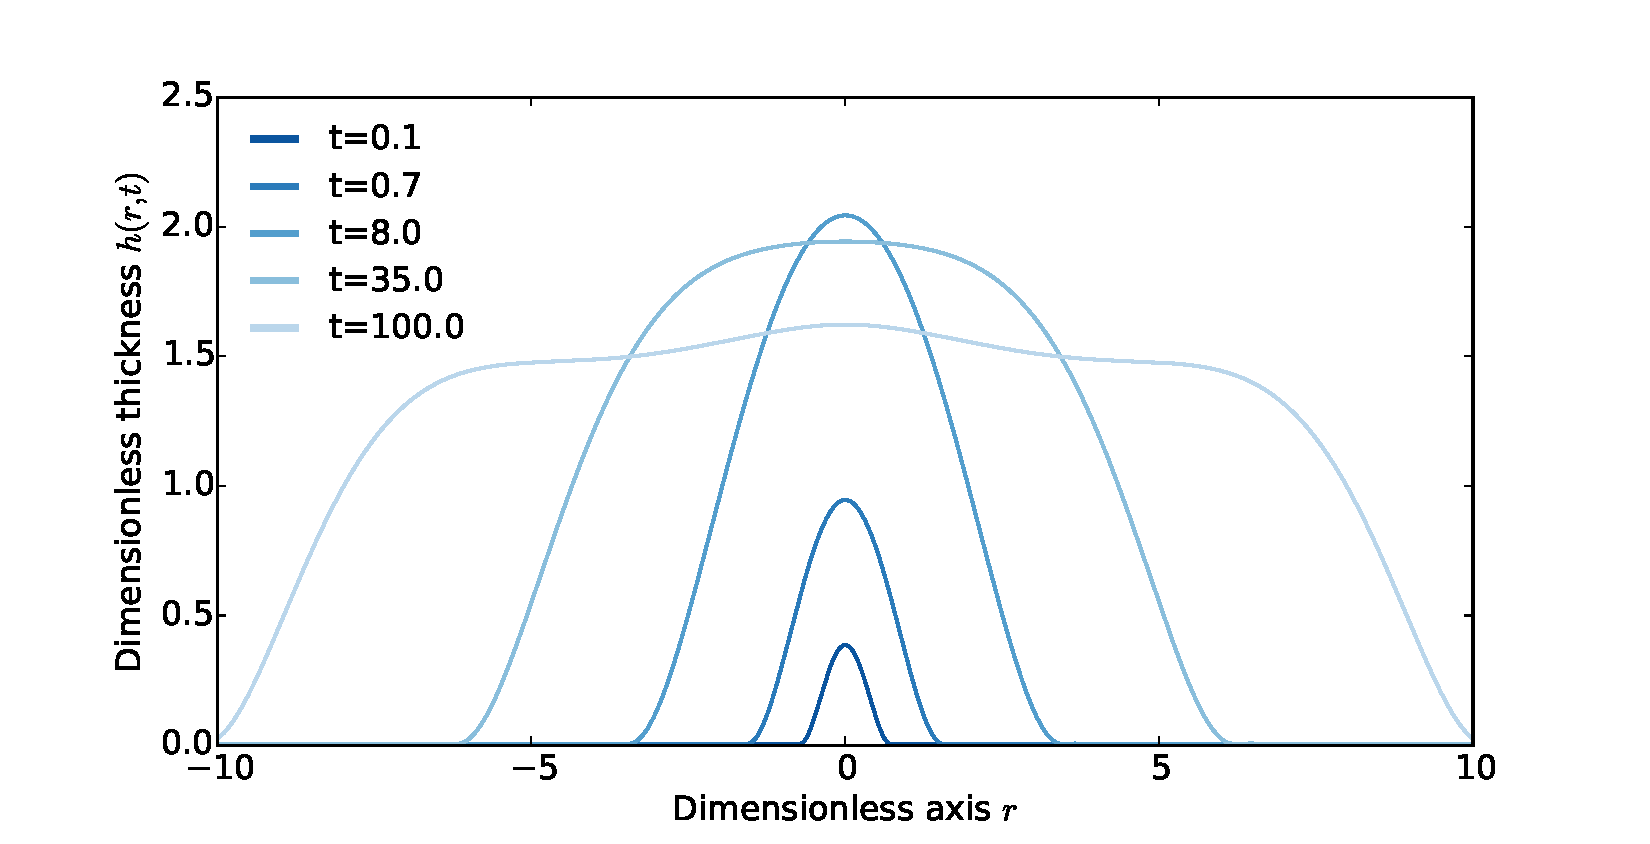
\includegraphics[scale=0.5]{C2_ELAS_GRAV_Profil.eps}
    \caption{Shape of the flow, i.e.  thickness $h(r,t)$ as a function
      of the radial axis $r$ at  five different times indicated on the
      plot. Variables are  dimensionless and one needs  to multiply by
      the characteristic  scales (thickness,  length or time  given by
      (\ref{C2-H1}),   (\ref{C2-L1})  or   (\ref{C2-T1}))  to   obtain
      dimensional values.  For $t<10$, the intrusion is in the bending
      regime  whereas  for $t>10$  the  intrusion  is in  the  gravity
      current regime.}
    \label{C2_ELAS_GRAV_Profil}
  \end{center}
\end{figure}

\subsection{Bending regime}
\label{C2-sec:bending-regime}

At  early times,  when  $R<<\Lambda$, gravity  is  negligible and  the
dynamics of  the spreading  is governed  by the  bending of  the upper
layer.   In addition,  if $h_0<<\sigma$,  the overpressure  $\Delta P$
driving the flow is much larger than  the weight of the blister at the
center and the injection rate can be considered constant.

In that case, the spreading is  very slow and the interior has uniform
dimensionless pressure $P =\nabla_r^4h$.   The flow is bell-shaped and
its thickness is given by
\begin{equation}
  h(r,t) = h_0(t)\left(1-\frac{r^2}{R^2(t)}\right)^2
  \label{C2-IntrusionShape}
\end{equation}
with $h_0(t)$  the thickness  of the intrusion  at the  center (Figure
\ref{C2_ELAS_GRAV_Profil},                                     $t<10$)
\citep{Michaut:2011kg,Lister:2013ia}.       In       this      regime,
\citet{Lister:2013ia} have  shown that the spreading  is controlled by
the propagation  of a peeling by  bending wave at the  intrusion front
with dimensionless velocity $c$
\begin{equation}
  c=    \frac{\partial             R}{\partial            t}             =h_f^{1/2}
  \left(\frac{\kappa}{1.35}\right)^{5/2}
  \label{C2-WaveVelocity}
\end{equation}
where  $\kappa  =  \partial^2  h/\partial r^2$  is  the  dimensionless
curvature  of  the  interior  solution.   Using  the  propagation  law
(\ref{C2-WaveVelocity})  and   the  form  of  the   interior  solution
(\ref{C2-IntrusionShape}), they find that the radius and the height of
the intrusion evolve following
\begin{eqnarray}
  R(t) &=& 2.2h_f^{1/22}t^{7/22}\label{C2-ScalingR}\\
  h_0(t)&=&0.7 h_f^{-1/11}t^{8/22}\label{C2-ScalingH}
\end{eqnarray}
where the numerical  pre-factors have been matched  to our simulations
(Figure \ref{C2_ELAS_GRAV_Sigma}) . The  bell-shaped morphology of the
flow in  this regime is  very close  to the dome-shaped  morphology of
solidified    laccoliths   (Figure    \ref{C1-picture}   c,    d,   e)
\citep{Michaut:2011kg}.

\begin{figure}
  \begin{center}
    \graphicspath{ {/Users/thorey/Documents/These/Manuscript/Figure/Chapter2/} }
    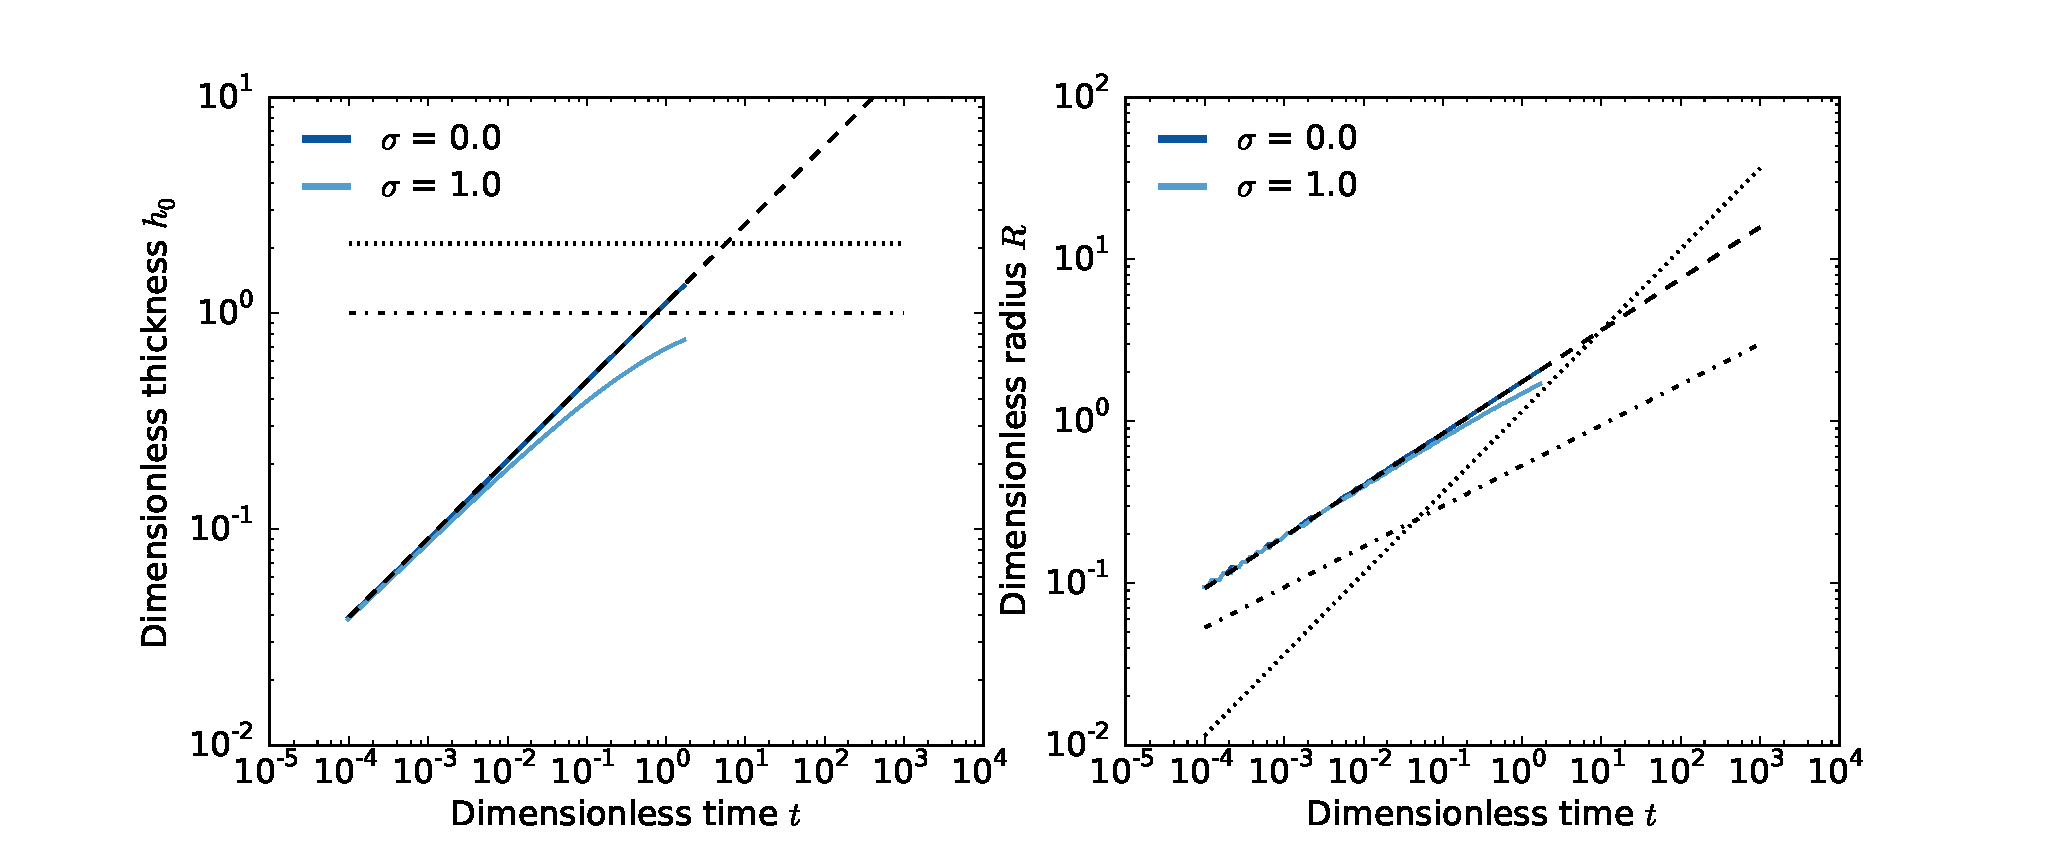
\includegraphics[scale=0.4]{C2_ELAS_GRAV_Sigma.eps}
    \caption{Left: Dimensionless thickness at  the center $h_0$ versus
      dimensionless  time  $t$  for  different  dimensionless  numbers
      $\sigma$  indicated on  the  plot.   Dashed-lines represent  the
      scaling  laws in  the different  regimes.  Right:  Dimensionless
      radius  $R$   versus  dimensionless   time  $t$  for   the  same
      dimensionless  number  $\sigma$.    Dashed-lines  represent  the
      scaling laws in the different regimes.}
    \label{C2_ELAS_GRAV_Sigma}
  \end{center}
\end{figure}

\subsection{Gravity current regime}
\label{C2-sec:grav-curr-regime}

In contrast,  when the radius  R becomes larger than  $\sim 4\Lambda$,
the weight of  the intrusion becomes dominant over  the bending terms.
The  dimensionless  pressure  is  given by  the  hydrostatic  pressure
$P = h$  and the intrusion enters a classical  viscous gravity current
regime where bending terms only affect the solution near the intrusion
edge         (Figure        \ref{C2_ELAS_GRAV_Profil},         $t>10$)
\citep{Huppert:1982a,Michaut:2011kg,Lister:2013ia}.   In  this  second
regime, while the thickness tends to be a constant, the radius evolves
as $t^{1/2}$ (Figure \ref{C2_ELAS_GRAV_Sigma}).  The flow is therefore
characterized by a small aspect-ratio $h_0/R$ and a constant thickness
disk-like  morphology close  to the  one  shown by  large mafic  sills
(Figure \ref{C1-picture} a).

In between the bending  and gravity regime, \citet{Lister:2013ia} also
describe  a short  intermediate regime  where the  peeling by  bending
continues to control the propagation  but where, due to the increasing
effect  of gravity,  the  flow shows  an  interior flat-topped  region
(Figure   \ref{C2_ELAS_GRAV_Profil},    $t=38$).    This   flat-topped
morphology     is     also     observed     in     many     laccoliths
\citep{Koch:1981if,Bunger:2011cb}.

\subsection{Lateral propagation}
\label{C2-sec:lateral-propagation}

Once $h_0\rightarrow \sigma$,  the flow is thick  enough to compensate
for  the initial  overpressure. The  thickness at  the center  remains
constant and  the flow enters  a regime of lateral  propagation, where
only its radius $R(t)$ increases \citep{Michaut:2011kg}. In this
regime, except at the center when it redistributes the pressure over a
length scale $\Lambda$, the bending term is negligible compared to the
gravitational  term. \citet{Michaut:2011kg}  has  shown  that in  this
regime, the thickness is constant and the radius evolves as $t^{1/4}$
\begin{eqnarray}
  R(t) &=& \left(\frac{\sigma^3 t}{4\pi}\right)^{1/4}\label{C2-Scaling-R-Propa}\\
  h_0 &=& \sigma\label{C2-Scaling-H-Propa}
\end{eqnarray} 

\section{Application to the spreading of shallow magmatic intrusions}
\label{C2-sec:appl-earth-moon}

\subsection{Observations versus predictions on Earth}
\label{C2-sec:observ-vs-pred}

\vspace{.5cm} \textbf{Dataset} \vspace{.5cm}

\citet{E:2015tl}  has made  an extensive  catalog of  $900$ laccoliths
across the  world.  In  particular, \citet{E:2015tl} provides  for the
thickness and  the radius  of $168$ laccoliths  among which,  $40$ are
also  given  with  an  estimation   of  the  intrusion  depth.   These
laccoliths,  who are  mainly felsic  in composition,  show thicknesses
that range from $100$ meters to $10$  km with radii in between $1$ and
$10$  km.  While  most of  the data  are located  in the  United State
($\sim 90\%$),  the different laccoliths  are widely spread  among the
territory  and   variations  in   the  parameters   between  different
laccoliths are most likely to be important.
\begin{figure}[h!]
  \begin{center}
    \graphicspath{ {/Users/thorey/Documents/These/Manuscript/Figure/Chapter2/} }
    \includegraphics[scale=0.35]{C2_Geological_Data.eps}
    \caption{a):  Cross section  of  western and  central Elba  Island
      where we can  see the christmas tree structure  of the laccolith
      complex and the main laccolith  units visible at the surface. b)
      Thickness  versus radius  of the  different laccolith  units. c)
      Sketch of the corresponding  location of these laccoliths within
      the    christmas   tree    structure    shortly   after    their
      formations. Figure modified from \citet{Rocchi:2002jy}.}
    \label{C2_Geological_Data}
  \end{center}
\end{figure}

Therefore,  in addition  to the  data from  \citet{E:2015tl}, we  also
consider in this  study the data provided  by \citet{Rocchi:2002jy} on
$9$ laccoliths  nested in a  christmas tree structure at  Elba Island,
Italy  (Figure \ref{C2_Geological_Data}).   The  detailed mapping  and
reconstruction  of  tectonic  history  made  by  \citet{Rocchi:2002jy}
provides for the  parameters of each intrusive layer  in the laccolith
complex. In  addition, for this dataset,  each laccolith is part  of a
larger intrusive system, and hence variability of the model parameters
should be limited,  except for the overlying  elastic layer thickness,
taken to be the intrusion depth, whose variation between laccoliths is
given by  \citet{Rocchi:2002jy}.  The  dispersion is much  smaller for
this dataset; the radius ranges from  $1$ to $10$ km and the thickness
from $40$ m to $1$ km.

Finally, we also account for  $25$ large mafic sills whose thicknesses
and radii are given by \citet{Cruden:tg}.  In order to account for the
intrinsic scale of  different settings for each  intrusion and compare
them to the model, the data  have first to be nondimensionalized using
characteristic  values for  each intrusion  parameters and  also their
depth, when absent from the catalog.

\begin{figure}[htpb]
  \begin{center}
    \graphicspath{ {/Users/thorey/Documents/These/Projet/Refroidissement/Skin_Model/Figure/Figure_Data/} }
    \includegraphics[scale=0.45]{Data_All_Squared.eps}
    \caption{a) Thickness  at the center  $h_0$ (m) versus  the radius
      $R$  (m)   for  magmatic  intrusions  from   different  datasets
      indicated on the plot. b)  Dimensionless thickness as a function
      of  dimensionless radius,  characteristic thickness,  and length
      are  calculated from  (\ref{C2-H1})  and (\ref{C2-L1}).   Dashed
      lines: predicted  scaling law  from the simulations  (black) and
      best fit for the power  law $h_0=aR^b$ for each dataset obtained
      from a  linear least-square regression in  log-log space.  $r^2$
      is  the squared  of the  correlation coefficient,  i.e.  Pearson
      product-moment correlation coefficient which gives an indication
      on the  goodness of the  fit; $1$ is total  positive correlation
      and $0$  is no correlation.   We use $\rho_m=2500$  kg m$^{-3}$,
      $Q_0 =2.5~10^3$ m$^3$ s$^{-1}$ and $\eta_h=10^6$ Pa s for felsic
      laccoliths  and  $\rho_m=2900$  kg m$^{-3}$,  $Q_0  =0.1$  m$^3$
      s$^{-1}$ and $\eta_h=10^2$  Pa s for large  mafic sills.  Unless
      the intrusion depth is given by the dataset, we use $d_c=1500$ m
      and $g=9.81$  m s$^{-2}$.  c)  and d),  same plots but  where we
      compared the  laccoliths from \citet{Rocchi:2002jy} to  a set of
      low-slope  lunar domes  given  by \citet{Wohler:2009jj}.   Lunar
      domes   are  nondimensionalized   using  $g=1.62$   m  s$^{-2}$,
      $\rho_m=3000$ kg  m$^{-3}$, $Q_0 =1$ m$^3$  s$^{-1}$, $\eta_h=1$
      Pa s  and $d_c$, which  is not given in  the dataset, is  set to
      $1500$ m. Purple dots correspond to morphometry reevaluated with
      the  LOLA  instrument topography  and  crosses  to the  original
      data. In all cases, the Poisson's ratio is $\nu^*=0.25$.}
    \label{C2-Corry_Rocchie}
  \end{center}
\end{figure}



\vspace{.5cm}   \textbf{Range   of    values   for   the   parameters}
\vspace{.5cm}

In terrestrial settings, magma density  $\rho_m$ mainly depends on its
composition and varies  between $ 2500$ kg m$^{-3}$  for felsic magmas
to  $2900$ kg  m$^{-3}$  for more  mafic  magmas.  Reported  intrusion
depths, which is set to $1.5$  km otherwise, vary from $180$ to $2200$
m for  laccoliths in \citet{E:2015tl} and  from $1.9$ to $3.7$  km for
laccoliths at Elba Island.  Hence, for a Young's modulus value of $10$
GPa, the characteristic length scale $\Lambda$ varies between $\sim 1$
km and $\sim  7$ km for laccoliths.  The density  does not affect much
the value of  $\Lambda$ and the characteristic length  scale for large
mafic sills,  whose depths are  not reported in  \citet{Cruden:tg} and
set to $1.5$ km, is equal to $\sim 3$ km.

On Earth, laccoliths are generally  formed by relatively evolved lavas
that  may have  differentiated from  primitive magma  in deep  crustal
magma chambers,  located some $5$  to $15$  km below the  surface. The
overpressures  driving magma  ascent are  typically $20$  to $50$  MPa
\citep{Stasiuk:1993kg,Barmin:2002ea},    which   gives    overpressure
gradients  of $\sim  10^3$ Pa  m$^{-1}$.  Lava  viscosity at  eruption
temperature  $\eta_h$  mainly depends  on  its  composition and  water
content; close to its liquidus  temperature, it can varies from $10^2$
Pa  s   for  mafic   lavas  to   $10^{6}$  Pa   s  for   felsic  lavas
\citep{Anonymous:CZVBrBvv,Giordano:2008em,Whittington:2009fv,Chevrel:2013jn}.
\citet{Wada:2007tv} shows that  the dyke width tends  to increase with
viscosity to  the power  $1/4$ \citep{Kerr:1995tl}; mafic  magmas with
viscosity $10^2$ Pa s at eruption  temperature tend to form dyke $1$ m
wide, while felsic  magmas, with viscosities of $10^6$-$10^7$  Pa s at
eruption temperature, tend  to form dykes $100$ m wide.   For the same
overpressure   gradient,  plugin   in   these   parameters  in   $Q_0$
(\ref{C2-eq11}) gives an injection rate  close to $0.1$ m$^3$ s$^{-1}$
for mafic magmas and $2.5~10^3$  m$^3$ s$^{-1}$ for felsic magmas. The
height  scale  $H$  is  thus  $\sim  25$  for  felsic  laccoliths  and
$\sim 0.1$ m for large mafic sills.

\begin{table}[h!]
  \caption{Range of values for the model parameters}
  \centering
  \begin{tabular}{c|c|c|c|c}
    Parameters& Symbol & Earth & Moon&Unit\\
    \hline
              &&&&\\
    Depth of intrusion & $d_c$ & $0.2-2.7$ &$1.5$ &km \\
    Young's Modulus & $E$ & $10$ &$10$ &GPa \\
    Poisson's ratio & $\nu^*$ & $0.25$ &$0.25$ &\\
    Gravity & $g$ & $9.81$ &1.62&m s$^{-2}$ \\
    Magma density & $\rho_{m}$ & $2500-2900$ &$2900$&kg m$^{-3}$ \\
    Magma viscosity & $\eta_h $ & $10^2-10^{6}$ &$1$&Pa s \\
    Feeder dyke width & $a$ & $1-100$ &$10$&m \\
    Depth of the melt source & $Z_{c}$ & $ 1-10$&$ 500$& km \\ 
    Initial overpressure & $\Delta P$ & $20-50$ &$50$ &MPa \\
    Injection rate & $Q_{0}$ &$0.1-10^3$ &$10^4$&m$^{3}$ s$^{-1}$ \\
              &&&&\\
    \hline
    Characteristic scales & Symbol & Earth & Moon&Unit\\
    \hline
              &&&&\\
    Height scale & $H$& $0.1-25$ &$2$ &m \\
    Length scale & $\Lambda$ & $1-7$&$3.3$& km \\
    Time scale & $\tau$ & $10^{-1}-10$&$10^{-2}$& years \\
    \label{C2-tab2}
  \end{tabular} 
\end{table}

The model  also considers  a thin pre-wetted  film of  thickness $h_f$
whose  meaning in  the application  to the  spreading of  laccolith is
unclear.  In  particular, the  model shows  no convergence  when $h_f$
tends to zero \citep{Lister:2013ia} and therefore, the thickness $h_f$
might be  linked to some structural  length scale at the  front of the
laccolith or  to the natural  imperfection of the flow  geometry.  For
the purpose of the application, we  choose a film thickness of $1$ mm,
i.e.   the minimum  length scale  with physical  significance for  the
spreading of laccoliths  which give a dimensionless  $h_f$ that varies
between $10^{-2}$  and $10^{-4}$.  In  the following, we set  $h_f$ to
$10^{-3}$.

\vspace{.5cm}  \textbf{Dimensionless  data  and  comparison  with  the
  model} \vspace{.5cm}

Each  magmatic   intrusion  unit  is  made   dimensionless  using  its
characteristic  length   scale  $\Lambda$,  which  depends   upon  the
intrusion depth, and its characteristic  height scale, which is either
$H=25$ m  for felsic  laccoliths or  $H=0.1$ m  for large  mafic sills
(Figure \ref{C2-Corry_Rocchie}).   First, the dimensionless  radius of
laccoliths at  Elba Island and  $95\%$ of those  from \citet{E:2015tl}
are  smaller than  $4$ consistent  with  their arrest  in the  bending
regime. The prediction of the model for the evolution of the thickness
$h_0$ of  the current as  a function of its  radius $R$ can  be easily
derived    from    the    scaling   laws    (\ref{C2-ScalingH})    and
(\ref{C2-ScalingR}) and should follow
\begin{equation}
  h_0 \sim 0.3h_f^{-1/7} R^{8/7}\label{C2-Hr}
\end{equation}
in agreement  with the power  law relationship $h_0 =  bR^a$ initially
proposed         by          \citet{McCaffrey:1997ea}         (Section
\ref{C1-sec:empl-dynam-des}).  To characterize the  mean trend in each
population, we use  a linear least-square regression  in log-log space
to obtain a  value for the coefficient  $a$ and $b$ that  best fit the
observations.  We found $h_0 = 21 R^{1.22}$ for the laccoliths at Elba
island  which is  very  close  to $R^{1.14}$  predicted  by the  model
(Figure \ref{C2-Corry_Rocchie},  $r^2=0.96$).  Actually,  the geometry
of  these laccoliths  is not  well  known and  probably not  perfectly
axisymmetric.   \citet{Anonymous:QWXp_4JV}   found  that  for   a  two
dimensional  flow, $h_0\propto  h_f^{-1/7}L^{10/7}$ where  $L$ is  the
half-length of the flow ($10/7\sim 1.43$).  The best fit value for the
coefficient $a$  then nicely inserts  between the expected  values for
the two  geometries as noted by  \citet{Michaut:2011kg}.  In contrast,
the prediction for the coefficient $b$  is much smaller than the value
derived from the observations.  Even for $h_f=10^{-2}$, which would be
an upper bound  for this parameter, the model  predict $b=0.15$, which
is three  orders of magnitudes  smaller than the  observations (Figure
\ref{C2-Corry_Rocchie}).  Matching the data  to the model will require
using  a  viscosity  $\eta_h$  for the  magma  abnormally  high,  i.e.
$\eta_h   \sim  10^{12}$   Pa  s   or  unreasonable   injection  rate,
i.e. $Q_0\sim 1$ km$^3$ s$^{-1}$.

The  best  fit   power  law  relationship  for   the  laccoliths  from
\citet{E:2015tl}     is     $h_0     =    21     R^{0.62}$     (Figure
\ref{C2-Corry_Rocchie}, $r^2  =0.54$). In that case,  the exponent $a$
is smaller than one and does not agree with the model.  This value for
$a$, slightly smaller  than the value calculated directly  on the data
by  \citet{McCaffrey:1997ea},   was  interpreted  as   reflecting  the
two-stage  growth process  historically invoked  for the  formation of
laccoliths   (Section   \ref{C1-sec:empl-dynam-des}).   However,   the
dispersion in the data is much more important than in the observation from
\citet{Rocchi:2010dn} and is not taken into account in the
nondimensionalization which  assumes the  same parameters for  all the
different  laccoliths. It  might explain  the discrepancy  between the
model prediction and the observation in this example.

Half of the  large mafic sills show dimensionless  radius smaller than
$R=4$, not consistent with their  arrest in the gravity current regime
(Figure \ref{C2-Corry_Rocchie}).   It might  suggest that  these mafic
sills  have  intruded shallower  into  the  crust; for  instance,  for
$d_c=250$ m,  the characteristic  length scale for  the mafic  sill is
smaller   $\Lambda=800$  m   and   $95\%$  of   the  population   show
dimensionless   radius   larger   than   $4$.    Nevertheless,   their
dimensionless  thickness, which  should tend  to a  constant of  order
$O(1)$ according to the model, is  much larger than the expected value
and increases  with the radius  $R$.  For a  gravity current in  a two
dimensional  geometry, the  thickness is  indeed expected  to increase
with the length  of the sill, but  as $L^{1/4}$ \citet{Michaut:2011kg}
which is much  weaker than the found value for  the coefficient $a$ of
$0.76$   for   large   mafic  sill   (Figure   \ref{C2-Corry_Rocchie},
$r^2=0.9$).  Therefore,  the model predictions hardly  reconcile with
the observations for large mafic sills.

\subsection{Origin of lunar low-slope domes}
\label{C2-sec:observ-vs-pred}

\vspace{.5cm}\hspace{.5cm} \textbf{Dataset} \vspace{.5cm}

On the Moon, $13$ elongated  low-slope domes, located around the lunar
maria, have  been recently  identified as potentially  intrusive domes
\citep{Wohler:2007it,Wohler:2009jj}.   \citet{Wohler:2009jj}  used  an
image-based $3D$ reconstruction approach which relies on a combination
of photoclinometry and shape from  shading techniques to determine the
morphometric properties of each of  these lunar domes which results in
a $10\%$  error estimate on  the intrusion thickness. These  data have
since  been updated  by Mélanie  Thiriet,  a graduate  student in  our
laboratory, who  used the high  resolution of the  topography obtained
from  the  $64$ ppd  ($\sim  450$  m/pixel \citep{Zuber:2009bq})  LOLA
gridded  topography data  downloaded  from the  planetary data  system
geosciences node to reevaluate the thickness and the radius of some of
these potentially intrusive lunar domes.

\vspace{.5cm} \textbf{Range of value for the parameters} \vspace{.5cm}

Given the basalt composition of most lunar rocks from the mare brought
back from the Apollo missions, the  lunar magmas are more likely to be
mafic in  composition and we use  $\rho_m = 2900$ kg  m$^{-3}$ for the
lava density. Therefore, on the Moon,  the larger lava density and the
smaller  gravity  leads  to  length  scale  $1.5$  times  larger  than
terrestrial ones. For  instance, using $E=10$ GPa and $d_c  = 1.5$ km,
the characteristic length  scale for a lunar intrusion is  $\sim 5$ km
and $3.3$ km for a terrestrial laccolith.

The source  of magma in the  lunar interior is poorly  constrained and
more likely to  be deeper than on  Earth; most of the  mare basalt are
thought to be a product of melting initiated deep in the lunar mantle,
deeper than $400$ km \citep{Shearer:2006gg}.  Using the same value for
the initial driving pressure, $\Delta P = 50$ MPa, unless lunar magmas
are  likely to  be  more  mafic and  contain  less volatiles  implying
smaller driving pressure, and a depth of $500$ km for the magma source
region, the overpressure  gradient is only of $100$  Pa m$^{-1}$. Mare
basalts, which  have lower concentration in  alkalies than terrestrial
basalts, should also have a lower  viscosity.  We take $\eta_h=1$ Pa s
and  for a  dyke  $10$ m  thick, the  injection  rate is  $Q_0=10^{4}$
m$^{3}$ s$^{-1}$ and the typical height scale $H\sim 2$ m .

\vspace{.5cm} \textbf{Predictions versus observations} \vspace{.5cm}

After   nondimensionalization,   the   lunar  low-slope   domes   show
dimensionless radius smaller than $4$  consistent with their arrest in
the bending  regime. In  addition, they  are almost  perfectly aligned
with   the   terrestrial   laccolith    from   Elba   Island   (Figure
\ref{C2-Corry_Rocchie}) \citep{Michaut:2011kg}.  Indeed,  the best fit
for all  the observations,  lunar domes +  Elba Island  laccoliths, is
$h_0   =    10R^{1.11}$   with   a   high    correlation   coefficient
$r^2=0.94$. Given that  the same intrusion depth  has been arbitrarily
chosen  for   all  intrusions,  the  fit   is  surprisingly  accurate.
Therefore,  the   isoviscous  elastic-plated  gravity   current  model
supports  the  intrusive  origin  of  the  lunar  domes  described  by
\citet{Wohler:2009jj}  and their  arrest  in the  bending regime.   In
addition,  it is able  to explain  the  difference between  Earth
laccolith and lunar intrusive domes \citep{Michaut:2011kg}.

\subsection{Discussion}
\label{C2-sec:discussion-1}

Historical models  for intermediate scale magmatic  intrusion consider
that  the main  phase  of  laccolith growth  and  spreading require  a
two-stage process: horizontal spreading of a sill followed by vertical
inflation  when the  sill has  grown horizontally  enough so  that the
magma has enough leverage on the overlying layer to begin to bend them
upward \citep{Johnson:1973ho,Koch:1981if}.  More recent models instead
proposed that  these intrusions form  as a series  of sub-horizontally
staked magma  sheets \citep{Morgan:2008hj,Menand:2011ki}.   While both
model are  able to account  for several geological  observations, they
both lack a physical description of the intrusion process and are then
not  able  to explain  the  solidified  morphology of  these  magmatic
intrusions in term of the  flow parameters (injection rate, volume) at
the time of emplacement.

\vspace{.5cm}   \textbf{Isoviscous  elastic-plated   gravity  current}
\vspace{.5cm}

\citet{Michaut:2011kg}  has   developed  a   new  approach   to  model
intermediate-scale intrusions such as  sills, laccoliths or bysmaliths
through a  dynamic elastic-plated gravity current  model that consider
both the bending and the own weight  of the magma as driving the flow.
This model shows promising results in predicting the variety of shapes
of  intermediate scale  magmatic intrusions;  from the  dome shape  of
laccolith to the disk-like morphology  of large mafic sill.  It allows
to relate the  laccolith morphology to the crustal  and magma physical
properties,  and  more  importantly,   to  the  injection  rate.   The
prediction of the model, especially  the scaling law for the thickness
versus length in the bending regime,  also fits the variability in the
laccolith  units  at  Elba  Island, hence  providing  for  a  physical
explanation for the observed relationship between laccolith length and
thickness. In  particular, it shows  that the main phase  of laccolith
growth and  spreading does  not require a  two-stage process  but that
spreading and thickening  simultaneously occur \citep{Michaut:2011kg}.
Finally,  the   model  shows  promising  results   in  explaining  the
discrepancy between terrestrial laccolith and low-slope lunar domes on
the Moon. Therefore,  it can be use to assess  the intrusive origin of
intrusive candidates on other terrestrial planets.

However, other questions  remain open.  First, we have  shown that the
model  hardly accounts  for  the  absolute final  value  for both  the
thickness and the  radius of these laccoliths  and that reconciliating
predictions and observations requires abnormally high magma viscosity.
Second, the  model was also  not able to  account for the  increase in
large mafic sill thickness with  their diameter. More importantly, the
model crucially  lack of a  stopping criterion that could  predict the
final morphology of  a magmatic intrusion given  its input parameters.
Fracturation is generally considered as  the limiting mechanism to the
expansion of magmatic intrusions.

\vspace{.5cm} \textbf{Criterion for fracturation} \vspace{.5cm}

As the flow length increases, the pressure in the intrusion eventually
decreases to  the critical value  equal to the pressure  necessary for
fracturing the  tip. In that case,  fracturing at the tip  might limit
spreading and trigger the arrest of a laccolith in the bending regime.
The  stress intensity  factor  $K_I$ for  a mode  $I$  fracture and  a
uniformly loaded crack situated close to a boundary (i.e., $d<<R$) can
be approximated by \citep{Dyskin:2000iz,Bunger:2005ee}
\begin{equation}
  K_I = K_M M_0 d_c^{-3/2}
  \label{C2-KC}
\end{equation}
where $K_M = 1.932$  is a constant and $M_0$ is  the bending moment at
the crack tip given by
\begin{equation}
  M_0        =        -D       \left.\left(\frac{\partial^2        h}{\partial
        r^2}+\frac{1}{r}\frac{\partial                     h}{\partial
        r}\right)\right|_{r=R(t)}.
  \label{C2-moment}
\end{equation}
Once  $K_I$   reaches  the   fracture  toughness  limit   $K_c$,  i.e.
$\sim 4-400$  MPa m$^{1/2}$  \citep{Olson:2003hca}, fracturing  at the
tip will limit the intrusion lateral extent.

Injecting the  scaling for the  thickness $h_0$  as a function  of the
radius $R$ (\ref{C2-Hr}) with dimension  into the predicted flow shape
in the  bending regime (\ref{C2-IntrusionShape}) gives  the flow shape
as a function of the radius $R(t)$ of the laccolith
\begin{equation}
  h(r,t) = 20 H \Lambda^{-8/7} R(t)^{8/7}\left(1-\frac{r^2}{R^2(t)}\right)^2.
\end{equation}
Injecting this expression into (\ref{C2-moment}) and (\ref{C2-KC}) and
inverting  for  the radius,  one  can  then  found that  the  critical
dimensionless radius $R_{cr}$ for the laccolith is
\begin{equation}
  R_{cr} \sim \frac{20 E^{7/6} H^{7/6} K_{m}^{7/6}}{K_{c}^{7/6} \Lambda^{7/3}} d^{7/4}
\end{equation}
which, in terms of the parameters, reads
\begin{equation}
  R_{cr} \sim 142 E^{7/12}K_{m}^{7/6} Q_{0}^{7/24} \eta_h^{7/24} g^{7/24} \rho_m^{7/24}}K_{c}^{-7/6}
\end{equation}
and therefore depends mainly in the fracture toughness of the encasing
rocks.  On can calculate that for typical crustal and magma parameters
taken   in   Section  \ref{C2-sec:appl-earth-moon}   for   terrestrial
laccoliths and the largest reported value for the parameter $K_c=4000$
MPa m$^{1/2}$, the critical dimensionless radius is equal to $\sim 10$
and therefore,  still much larger  than the transition  radius between
the bending and gravity regime  $R= 4$.  Therefore, while fracturation
might explain the  arrest of magmatic intrusion for  large mafic sill,
it  does  not  provide  a  sufficient  mechanism  for  the  arrest  of
laccolith.

\section{Toward   a  more   realistic  model   for  shallow   magmatic
  intrusions}
\label{C2-sec:discussion}

We have shown that while it shows promising results in reproducing the
morphology of  solidified magmatic intrusions  on Earth and  the Moon,
the isoviscous elastic-plated gravity current suffers some limitations
as  well.  In  this manuscript,  we propose  to explore  two important
mechanisms  that have  been  neglected until  now  and will  certainly
influence the emplacement of shallow  magmatic intrusions in the crust
of terrestrial  planets: the  effect a  temperature-dependent rheology
for  the magma  and the  effect of  an overburden  characterized by  a
non-constant thickness.

The former has already shown important implications for the cooling of
lava                                                             domes
\citep{Bercovici:2007vc,Bercovici:1996uu,BALMFORTH:1999ey,Garel:2014era}. Indeed,
the viscosity of magma can vary by several orders of magnitudes during
the  cooling \citep{Anonymous:CZVBrBvv,Lejeune:1995fc}  and therefore,
as the fluid cools, its  composition and crystal content change which,
in  turn,  modifies  the  viscosity  and  the  dynamics  of  the  flow
itself. The  first part of the  manuscript deals with this  matter and
try  to better  understand the  dynamics of  a cooling  elastic-plated
gravity current.  In particular, in chapter  $3$, we derive a model of
a cooling  elastic-plated gravity  current with a  viscosity inversely
dependent  on temperature  and isothermal  boundary conditions.   This
model  is next  further refined  and  compared to  the observation  in
chapter $4$.

The second  part of the manuscript  addresses the second point  and in
particular, the problem of crater-centered intrusions with application
to  the  endogenous  deformation  observed  at  lunar  floor-fractured
craters.  Indeed, if  large volume of magma  have effectively intruded
at   shallow    depth   below    these   craters   as    proposed   by
\citet{Schultz:1976kt}, the  topography of  the initial  impact crater
has to constrain the underlying  magma spreading dynamics. Chapter $5$
presents a model for crater-centered intrusions and its application to
the  deformations  observed   at  floor-fractured  craters.   Finally,
chapter  $6$  takes the  study  of  floor-fractured craters  one  step
further   by  looking   at  the   gravitational  signature   of  lunar
floor-fractured craters in the light of the model predictions.

This  approach, evolving  each time  from a  theoretical model  to the
observations, might  help shed  light both on  the limitations  of the
model of \citet{Michaut:2011kg} exposed in this chapter and the origin
of lunar-floor fractured craters.

\newpage
\bibliographystyle{agufull08}
\bibliography{/Users/thorey/Dropbox/Library}



%%% Local Variables:
%%% mode: latex
%%% TeX-master: "../main"
%%% End:
